\documentclass[a4paper,12pt]{article}

\usepackage[utf8]{inputenc}
\usepackage[T1]{fontenc}
\usepackage[english]{babel}
\usepackage{csquotes}
\usepackage{microtype} 
\usepackage{stmaryrd}
\usepackage[a4paper, left=1.75cm, right=1.75cm, top=2.5cm, bottom=2.5cm,
            heightrounded, headheight=14pt, headsep=12pt]{geometry}

\usepackage{amsmath,amsfonts,amssymb,mathtools,bm}

\usepackage{graphicx}
\usepackage{float}
\usepackage{multirow}
\usepackage{booktabs}
\usepackage{tabularx}
\usepackage{array}                       
\newcolumntype{Y}{>{\centering\arraybackslash}X}
\usepackage[justification=centering,skip=10pt,font=small,labelfont=bf]{caption}
\usepackage{subcaption}
\usepackage{ragged2e}                   
\graphicspath{{results/}{figures/}{Page_Garde/}}

\usepackage[table,xcdraw]{xcolor}
\definecolor{codegreen}{rgb}{0,0.6,0}
\definecolor{codegray}{rgb}{0.5,0.5,0.5}
\definecolor{codepurple}{rgb}{0.58,0,0.82}
\definecolor{backcolour}{rgb}{0.95,0.95,0.92}

\usepackage{listings}
\lstdefinestyle{mystyle}{
  backgroundcolor=\color{backcolour},
  commentstyle=\color{codegreen},
  keywordstyle=\color{magenta},
  numberstyle=\tiny\color{codegray},
  stringstyle=\color{codepurple},
  basicstyle=\ttfamily\footnotesize,
  breakatwhitespace=false,
  breaklines=true,
  captionpos=b,
  keepspaces=true,
  numbers=left,
  numbersep=5pt,
  showspaces=false,
  showstringspaces=false,
  showtabs=false,
  tabsize=2,
  language=Python
}
\lstset{style=mystyle}

% ---------- liens ------------------------------------------------------------
\usepackage[hidelinks]{hyperref}
\usepackage{cleveref}

% ---------- espacements (style du 2e template) -------------------------------
\usepackage{titlesec}
\usepackage{enumitem}
\usepackage{setspace}
\setlength{\parskip}{1em}      % espace entre paragraphes
\setlength{\parindent}{0pt}    % pas d'indentation
\linespread{1}              % interligne
\titlespacing*{\section}{0pt}{0.5em}{0.5em}
\titlespacing*{\subsection}{0pt}{0.5em}{0.5em}
\titlespacing*{\subsubsection}{0pt}{0.5em}{0.5em}
\setlist{itemsep=5pt, parsep=5pt, topsep=5pt}

\newcommand{\reporttitle}{Recognizing Handwritten Digits by Optimization:}
\newcommand{\reportsubtitle}{Fitting a Regularized Smoothed-Hinge Linear
Classifier with Fixed-Step Gradient Descent}
\newcommand{\documenttype}{Homework 1 Report}
\newcommand{\coursename}{MATH-329 -- Continuous Optimization}

\newcommand{\groupmembers}{%
  Tara \textsc{Davies} \\
  Noalynne \textsc{Deker} \\
  Victor \textsc{Hubert} \\
  Boray \textsc{Kasap}
}
\newcommand{\institution}{\'Ecole Polytechnique F\'ed\'erale de Lausanne}
\newcommand{\reportdate}{\today}
\newcommand{\academicyear}{2026-2027}

\usepackage{fancyhdr}
\pagestyle{fancy}
\fancyhf{}
\fancyhead[L]{\footnotesize\coursename}
\fancyhead[C]{}
\fancyhead[R]{\footnotesize Group X}
\fancyfoot[L]{\footnotesize EPFL}
\fancyfoot[C]{\footnotesize\thepage}
\fancyfoot[R]{\footnotesize\academicyear}
\renewcommand{\headrulewidth}{0.4pt}
\renewcommand{\footrulewidth}{0.4pt}


%  MACROS

\newcommand{\R}{\mathbb{R}}
\newcommand{\E}{\mathcal{E}}
\newcommand{\vecop}{\operatorname{vec}}
\newcommand{\xt}{\tilde{x}}
\newcommand{\Xt}{X}
\newcommand{\inner}[2]{\left\langle #1,\,#2\right\rangle}
\DeclarePairedDelimiter{\norm}{\lVert}{\rVert}
\newcommand{\grad}{\nabla}
\newcommand{\smax}{\sigma_{\max}}

\begin{document}

\begin{titlepage}
\newcommand{\HRule}{\rule{\linewidth}{0.5mm}}
\center

\includegraphics[width=0.5\linewidth]{figures/epfl-logo.png}\\[1cm]

\HRule \\[0.5cm]
{\huge \bfseries \MakeUppercase{\documenttype}}
\HRule \\[0.8cm]

\begin{minipage}{1\textwidth}
\centering
\resizebox{\linewidth}{!}{\scshape\reporttitle}\\[0.2cm]
\textsc{\large \reportsubtitle}
\end{minipage}\\[0.8cm]

\includegraphics[width=\linewidth]{figures/trial.png}\\[0.8cm]


\textsc{\large Course:}\\
\textsc{\coursename}\\[0.5cm]

\textsc{\large Group:}\\
\fancyhead[R]{\footnotesize Group X}.

\textsc{\large Students:}\\
\begin{tabular}{@{}c@{}}\groupmembers\end{tabular}\\[0.5cm]

\textsc{\large Date:}\\
\textsc{\reportdate}

\end{titlepage}

\setcounter{page}{1}


\section{Existence and uniqueness}\label{sec:q1}

$\phi$ \textbf{is differentiable.}
On each of the intervals $\left]-\infty,-1\right]$, $[-1,0]$ and $\left[0,+\infty\right[$, $\phi$ coincides with a polynomial, so it is differentiable on the corresponding open intervals. At the junction points $-1$ and $0$, the polynomials on either side agree, and so do their derivatives: each one-sided derivative is that of the polynomial on that side, and at $-1$ both equal $0$, at $0$ both equal $1$.
Hence $\phi$ is differentiable on all of $\R$, with, for all $z \in \R$,
\[
  \phi'(z) =
  \begin{cases}
    0      & \text{if } z \le -1, \\[2pt]
    1 + z  & \text{if } -1 \le z \le 0, \\[2pt]
    1      & \text{if } 0 \le z .
  \end{cases}
\]

$\phi$ \textbf{is convex.}
We use Lemma~4.22. Let $x,y \in \R$. The case $x=y$ is trivial, so suppose $x \neq y$.
By the mean value theorem there exists $c$ strictly between $x$ and $y$ with $\phi(y) - \phi(x) = \phi'(c)(y-x)$.
Since $\phi'$ is non-decreasing (see the formula above), $\phi'(c) \geq \phi'(x)$ when $y>x$ and $\phi'(c) \leq \phi'(x)$ when $y<x$; in both cases $\phi'(c)(y-x) \geq \phi'(x)(y-x)$. Hence $\phi(y) \geq \phi(x) + \phi'(x)(y-x)$, so $\phi$ is convex by Lemma~4.22.

\textbf{Deduce} $f_{\lambda}$ \textbf{strongly convex and differentiable.}
For each $i \in \llbracket 1,m \rrbracket$, the map $\theta \mapsto \phi(s_i \xt_i^\top \theta)$ is convex on $\E$, as the composition of the convex function $\phi$ with an affine map (Exercise~4.17).
A non-negative combination of convex functions is convex (Exercise~4.13), so $f(\theta) = \sum_{i=1}^m \phi(s_i \xt_i^\top \theta)$ is convex.
Since $f_{\lambda}(\theta) - \tfrac{\lambda}{2}\norm{\theta}^2 = f(\theta)$ is convex and $\lambda > 0$, $f_{\lambda}$ is $\lambda$-strongly convex by definition.
Moreover, $f_{\lambda}$ is differentiable, as a sum of compositions of the differentiable function $\phi$ with affine maps and of the quadratic $\theta \mapsto \tfrac{\lambda}{2}\norm{\theta}^2$.

\textbf{Deduce} $f_{\lambda}$ \textbf{has a unique critical point.}
Since $f_{\lambda}$ is strongly convex, it admits exactly one global minimizer $\theta^\star \in \E$ (Theorem~4.28).
Since $f_{\lambda}$ is moreover convex and differentiable, Corollary~4.23 tells us that $\theta \in \E$ is a global minimizer of $f_{\lambda}$ if and only if $\nabla f_{\lambda}(\theta) = 0$.
Combining the two, the set of critical points of $f_{\lambda}$ is exactly the set of global minimizers, which is the singleton $\{\theta^\star\}$.

\medskip
\noindent\textit{From here on we fix $\lambda = 0.005$.}
% =============================================================================
\section{Objective and gradient}\label{sec:q2}
% -----------------------------------------------------------------------------

\subsection{Derivation}
We write $f(\theta) = \displaystyle \sum_{i=1}^m \phi(g_i(\theta))$ and $f_{\lambda}(\theta) = f(\theta) + h(\theta)$, with $g_i(\theta) = s_i \langle \xt_i,\theta \rangle$ for $i \in \llbracket 1,m\rrbracket$ and $h(\theta) = \frac{\lambda}{2}\norm{\theta}^2$, for $\theta \in \E$.

In what follows, $\theta, v \in \E$ are arbitrary.

\textbf{We compute} $\grad h$.
We have:
\begin{align*}
Dh(\theta)[v] &= \lim_{t\to 0} \frac{h(\theta + tv) - h(\theta)}{t} \\
      &= \frac{\lambda}{2} \lim_{t\to 0} \frac{\langle \theta + tv, \theta +tv \rangle - \langle \theta, \theta \rangle}{t} \\
      &= \frac{\lambda}{2} \lim_{t\to 0} \big( 2\langle \theta, v \rangle + t\langle v, v \rangle \big) \\
      &= \langle \lambda \theta, v \rangle.
\end{align*}
Hence $\grad h(\theta) = \lambda \theta$.

\textbf{We compute} $\grad g_i$ \textbf{for} $i\in \llbracket 1,m\rrbracket$.
We have:
\begin{align*}
    D g_i(\theta)[v] &= \lim_{t\to 0} \frac{g_i(\theta + tv) - g_i(\theta)}{t} \\
                     &= \lim_{t\to 0} \frac{s_i \langle \xt_i, \theta + tv\rangle - s_i \langle \xt_i, \theta \rangle}{t} \\
                     &= \langle s_i \xt_i, v\rangle.
\end{align*}
Hence $\grad g_i(\theta) = s_i \xt_i$.

\textbf{We compute} $\grad f$.
By the chain rule and linearity of the differential,
\begin{align*}
   Df(\theta)[v] &= \sum_{i=1}^m D\phi(g_i(\theta))\big[D g_i(\theta)[v]\big] \\
                 &= \sum_{i=1}^m \phi'(s_i \langle \xt_i, \theta \rangle)\, s_i \langle \xt_i,v\rangle \\
                  &= \Big\langle \sum_{i=1}^m \phi'(s_i \langle \xt_i, \theta \rangle)\, s_i \xt_i,\ v \Big\rangle.
\end{align*}
Hence $\grad f(\theta) = \displaystyle \sum_{i=1}^m \phi'(s_i \langle \xt_i, \theta \rangle)\, s_i \xt_i$.

\textbf{We compute} $\grad f_{\lambda}$.
Again by linearity,
\begin{align*}
\grad f_{\lambda}(\theta) = \grad f(\theta) + \grad h(\theta) = \sum_{i=1}^m \phi'(s_i \langle \xt_i, \theta \rangle)\, s_i \xt_i + \lambda \theta
\end{align*}
For computations purposes, we will rewrite the gradient to use more of numpy's matrix multiplication. 
We place ourselves in the computation situation, i.e we consider that $\tilde{x_i} \in \mathbb R^{d+1}$, and $\theta \in \mathbb R^{d+1}$. 
We extend $\phi'$ to $\mathcal E$, where we apply the function to each component of the input vector.
Let $\tilde{X} = (\tilde{x}_1, ..., \tilde{x}_m) \in \mathbb R^{d+1 \times m}, s = (s_1,...,s_m)^\top \in \mathbb R^m$.
We then have : 
\begin{align*}
    \grad f_{\lambda}(\theta) &= \sum_{i=1}^m \phi'(s_i \langle \tilde{x_i}, \theta \rangle) s_i \tilde{x_i} + \lambda \theta \\ 
                              &= \tilde X (s\odot \phi'(s \odot (\tilde{X}^\top \theta))) + \lambda \theta 
\end{align*}


\subsection{Implementation and verification}
We compare the non-vectorized and vectorized implementations on the same random $\theta$, computing their relative difference. 
We obtain for $f_\lambda$ and $\grad f_\lambda$ a relative error of approximately $7.2\times10^{-16}$ and $3.2\times10^{-14}$ respectively. Both errors are at the level of floating-point rounding, which is expected since the two versions sum the $m$ terms in a different order, so the implementations agree up to numerical precision.

We time both versions on the same data, averaging $50$ runs timed with Python's \texttt{time.perf\_counter()}. 
The loop takes $0.1560$s, and the vectorized version $0.0098$s, i.e.
about $16\times$ faster. 
This is because the loop redoes the same small computation $m$ times in Python, which is slow, while the vectorized version does the same total amount of work using NumPy's fast, precompiled
array operations.

% =============================================================================
\section{Gradient check}\label{sec:q3}
% -----------------------------------------------------------------------------

We take $\theta$ as a random vector (fixed seed, small entries) and $v$ as a
random direction normalized to $\|v\|=1$. The resulting plot is shown in
Figure~\ref{fig:q3}; the straight portion has slope $\approx 2$. This
supports the correctness of our gradient, since a wrong gradient would
generically not produce this slope-2 behavior together with the flattening
at small $t$ (floating-point noise floor). It does not prove correctness:
the check only compares the gradient against a finite-difference
approximation along one direction $v$, so it could in principle miss an
error that happens to vanish along that particular direction.

\begin{figure}[H]
  \centering
  \IfFileExists{results/q3_gradient_check.pdf}
    {\includegraphics[width=0.4\linewidth]{results/q3_gradient_check.pdf}}
    {\fbox{\parbox[c][3cm][c]{0.4\linewidth}{\centering\ttfamily\small
      results/q3\_gradient\_check.pdf\\ (generated by \texttt{main})}}}
  \caption{Gradient check: the Taylor residual against the step size $t$, in
log--log coordinates; the linear portion has slope $\approx 2$.}
  \label{fig:q3}
\end{figure}


% =============================================================================
\section{Fixed-step gradient descent}\label{sec:q4}
% -----------------------------------------------------------------------------

We take the constant step size $\alpha = 1/L$, with
$L = \smax(X)^2 + \lambda$ as given. Rather than computing an SVD of
$X$ ($785 \times 12\,665$), we get $\smax(X)^2$ as the largest
eigenvalue of $XX^\top$ ($785 \times 785$), since the eigenvalues of $XX^\top$
are the squared singular values of $X$, and the smaller matrix is much cheaper
to form and diagonalize. This gives $L \approx 7.94\times10^5$ and
$\alpha = 1/L \approx 1.26\times10^{-6}$, which is a standard, easy-to-justify
pragmatic choice: it is the largest step size guaranteed safe for an
$L$-smooth objective, so we can use it without tuning.


% =============================================================================
\section{Run}\label{sec:q5}
% -----------------------------------------------------------------------------
We used a logarithmic vertical axis for both panels, as both quantities vary over several orders of magnitude during the run of fixed-step gradient descent.
On a linear scale, the objective curve $f_\lambda(\theta_k)$ would appear almost flat after the first few iterations, the initial drop dominating the vertical range and the following descent becoming visually indistinguishable from a horizontal line. This hides the curvature of the trajectory and makes the transition between the fast initial phase and the slower one unreadable, whereas a logarithmic scale preserves both regimes.
The same holds for the gradient norm $\norm{\grad f_\lambda(\theta_k)}$: on a linear plot, the curve would drop sharply and collapse onto zero, making the convergence rate impossible to read.

A linear axis would therefore hide essential structure of both curves, whereas the logarithmic axis reveals the convergence behavior: an early steep descent, followed by a slow phase, and the rate at which the gradient norm approaches zero.

\begin{figure}[H]
  \centering
  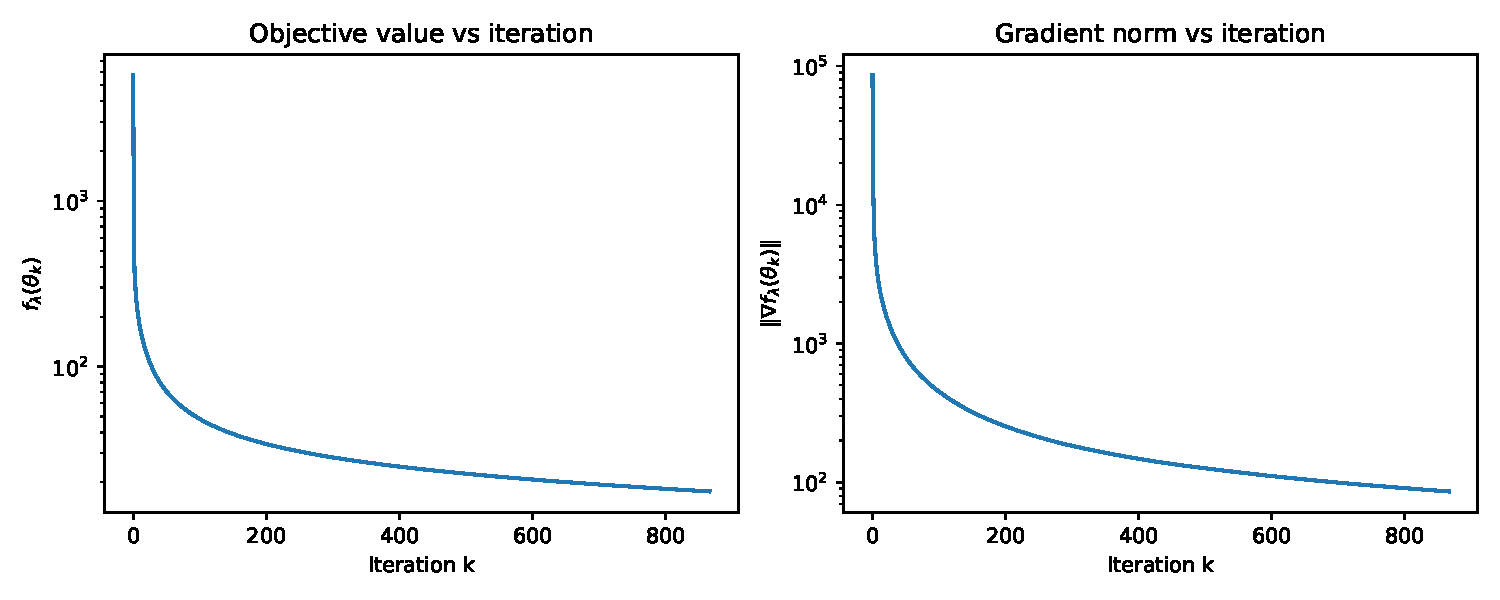
\includegraphics[width=\linewidth]{results/q5_convergence.pdf}
  \caption{Objective value (left) and gradient norm (right) against the
  iteration count $k$ for fixed-step gradient descent on $f_\lambda$.}
  \label{fig:q5}
\end{figure}

% =============================================================================
\section{Interpretation}\label{sec:q6}
\textbf{Strongest applicable result.} The sequence is $\theta_{k+1} = \theta_k - \alpha \nabla f_\lambda(\theta_k)$ with a fixed $\alpha > 0$. The strongest result in the lecture notes for such an iteration is Theorem~4.31: if $f$ is $\mu$-strongly convex with $L$-Lipschitz gradient and $\kappa = L/\mu$, then for any $\theta_0$, GD with step size $1/L$ satisfies
\[
  f(\theta_k) - f(\theta^\star) \le \Big(1 - \tfrac{1}{\kappa}\Big)^k \big(f(\theta_0) - f(\theta^\star)\big),
\]
i.e.\ the optimality gap converges at least linearly to $0$, from any starting point. 

\textbf{Assumptions and step size.} Both hypotheses hold for $f_\lambda$: it is $\mu$-strongly convex with $\mu = \lambda = 0.005$ (Question~1), and its gradient is $L$-Lipschitz with $L = \sigma_{\max}(X)^2 + \lambda$ (given). The theorem is stated for the step size $1/L$ exactly; Question~4 uses $\alpha = 1/L$ with $L = 7.94286 \times 10^5$, i.e.\ $\alpha = 1.25899 \times 10^{-6}$, so it applies to our choice.

\textbf{Prediction versus observation.} The condition number is $\kappa = L/\mu \approx 1.59 \times 10^8$, so the guaranteed contraction factor per iteration is $1 - 1/\kappa \approx 1 - 6.3 \times 10^{-9}$. The theorem thus predicts that the optimality gap converges linearly to $0$, but so slowly that over our $K = 867$ iterations it only guarantees a reduction by a factor $(1-1/\kappa)^{866} \approx 0.999995$. The run does far better: $f_\lambda$ fell from $5730.1$ to $17.63$, so, since $f^\star \ge 0$, the gap $f_\lambda(\theta_k) - f^\star$ shrank by a factor of at least $5730.1/17.63 \approx 325$; moreover, both curves in Figure~\ref{fig:q5} are concave rather than straight, a fast initial decrease that keeps slowing down.
% =============================================================================

\section{Does the classifier work?}\label{sec:q7}
Using the final iterate $\theta_{\mathrm{final}}$ from the run of Question~5, we classify each sample according to the prescribed rule: label $1$ when $\xt_i^\top\theta_{\mathrm{final}}>0$ and label $0$ otherwise. The final row of both \texttt{train.X} and \texttt{test.X} is already all ones, so no additional constant was appended.
The resulting classification error rates are given in Table~\ref{tab:q7}.

\begin{table}[H]\centering\small
\begin{tabular}{lrrr}
\toprule
 & Samples & Misclassified & Error rate \\
\midrule
Train & 12\,665 & 8 & $6.32\times10^{-4}$ \\
Test  & 2\,115  & 1 & $4.73\times10^{-4}$ \\
\bottomrule
\end{tabular}
\caption{Classification error of $\theta_{\mathrm{final}}$.}
\label{tab:q7}
\end{table}

The test error ($2\,115$ samples) is of the same order of magnitude as the training error ($12\,665$ samples). This indicates that the predictor obtained by fixed-step gradient descent generalizes well: it does not overfit the training data and maintains its performance on unseen samples. The test error is in fact slightly lower than the training error, but this should not be over-interpreted: it corresponds to a single misclassified test image out of $2\,115$, so a second misclassified image would already double it. The two error rates are therefore indistinguishable given the size of the test set, and the only conclusion we draw is that the classifier performs as well on unseen samples as on the training set.

% 
% =============================================================================
\section{What we learned}\label{sec:q8}
On the mathematical side, we learned that the regularization term $\tfrac{\lambda}{2}\norm{\theta}^2$ does a lot of work: without it, $f$ is only convex and may not even have a minimizer, while with it $f_\lambda$ is $\lambda$-strongly convex, so the minimizer exists, is unique, is the only critical point, and gradient descent is guaranteed to converge linearly. On the computational side, the loop and vectorized versions compute the same thing (they agree to $10^{-14}$) but the vectorized one is about $15\times$ faster, so the way a formula is implemented matters as much as the formula itself. The gradient check was also useful: it is cheap and catches a wrong gradient before it breaks the rest of the homework, even if it does not prove correctness. Finally, experimentally, the run showed us that Theorem~4.31 is a worst-case bound, not a prediction. With $\kappa \approx 1.6\times10^{8}$ it guarantees almost nothing over $866$ iterations, but the objective still dropped by a factor above $300$.

\end{document}
